\documentclass[letter,12pt]{article}
\usepackage[T1]{fontenc}
\usepackage[utf8]{inputenc}
\usepackage{lmodern}
\usepackage{hyperref}
\usepackage[english]{babel}
\usepackage{fourier}
\usepackage[protrusion=true,expansion=true]{microtype}
\usepackage{amsmath,amsfonts,amsthm}
\usepackage[pdftex]{graphicx}
\usepackage{sectsty}								
\usepackage[svgnames]{xcolor}			
%\allsectionsfont{\centering \normalfont\scshape}	
\usepackage{fancyhdr}
\pagestyle{fancyplain}
\fancyhead{}	
\fancyfoot[L]{\small \url{http://toddvance.tech}}		
\fancyfoot[C]{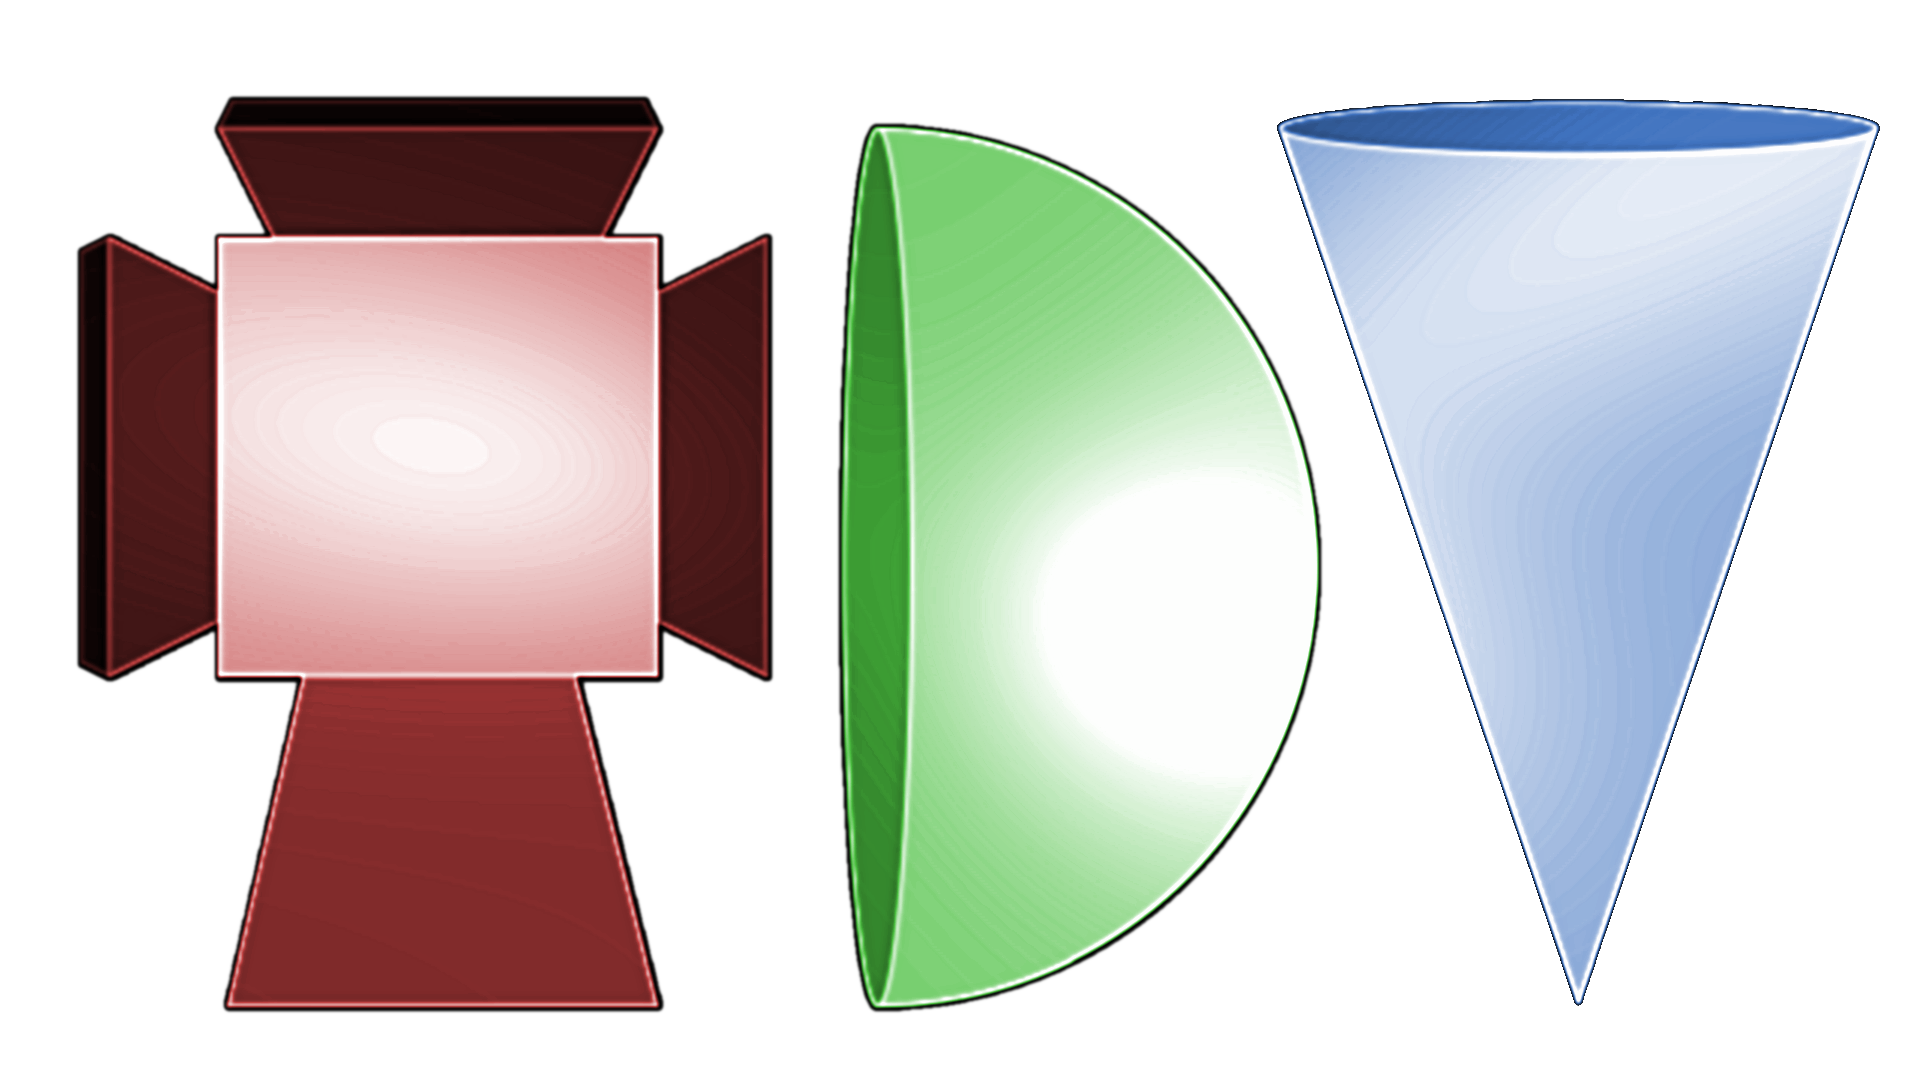
\includegraphics[width=0.5in]{common/monogram-transparent.png}}											
\fancyfoot[R]{\thepage}								
\renewcommand{\headrulewidth}{0pt}			
\renewcommand{\footrulewidth}{0pt}
\setlength{\headheight}{13.6pt}
\newcommand{\horrule}[1]{\rule{\linewidth}{#1}} 	% Horizontal rule

\title{
		%\vspace{-1in}
		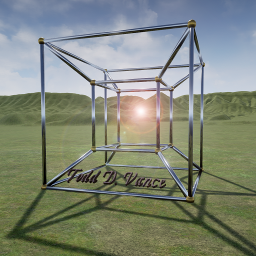
\includegraphics[width=1.5in]{common/tdv-logo-south-branch-valley-small.png}
		\usefont{OT1}{bch}{b}{n} 
		\normalfont 
		\horrule{0.5pt} \\[0.4cm]
		\Huge Quaternions and Rotations\\ %%%%%%%%%%%%%% TITLE %%%%%%%%%%%%%%%
		\color{DarkGreen}
		\large How To\\[0.2cm]%%%%%%%%%%%%%%ARTICLE TYPE %%%%%%%%%%%%%%%
		\color{Blue}
		\small \textsc{What are they and how do they work}\\%%%%%%%%%%%%%% TAG LINE %%%%%%%%%%%%%%%
		\color{Black}
		\horrule{2pt} \\[0.5cm]
}
\author{
		\normalfont \normalsize
       \copyright{2017 Todd D. Vance, Deplorable Mountaineer}%%%%%%%%%%%%%% COPYRIGHT %%%%%%%%%%%%%%%
        \tiny\\
\tiny        Permission is hereby granted, free of charge, to any person obtaining a copy\\[-0.3cm]
\tiny        of this software and associated documentation files (the "Software"), to deal\\[-0.3cm] 
\tiny        in the Software without restriction, including without limitation the rights to\\[-0.3cm]
\tiny         use, copy, modify, merge, publish, distribute, sublicense, and/or sell copies\\[-0.3cm] 
\tiny         of the Software, and to permit persons to whom the Software is furnished to\\[-0.3cm]
\tiny         do so, subject to the following conditions:\\[-0.3cm]
\tiny         \\[-0.3cm]
\tiny	The above copyright notice and this permission notice shall be included in all\\[-0.3cm]
\tiny	copies or substantial portions of the Software.\\[-0.3cm]
\tiny	\\[-0.3cm]
\tiny	THE SOFTWARE IS PROVIDED "AS IS", WITHOUT WARRANTY OF ANY KIND,\\[-0.3cm]
\tiny	EXPRESS OR IMPLIED, INCLUDING BUT NOT LIMITED TO THE WARRANTIES\\[-0.3cm] 
\tiny	OF MERCHANTABILITY, FITNESS FOR A PARTICULAR PURPOSE AND\\[-0.3cm]
\tiny	NONINFRINGEMENT. IN NO EVENT SHALL THE AUTHORS OR COPYRIGHT\\[-0.3cm]
\tiny	HOLDERS BE LIABLE FOR ANY CLAIM, DAMAGES OR OTHER LIABILITY,\\[-0.3cm]
\tiny	WHETHER IN AN ACTION OF CONTRACT, TORT OR OTHERWISE, ARISING\\[-0.3cm]
\tiny	FROM, OUT OF OR IN CONNECTION WITH THE SOFTWARE OR THE USE\\[-0.3cm]
\tiny   OR OTHER DEALINGS IN THE SOFTWARE.
}
\date{\today}

\newtheorem{exercise}{Exercise}

\begin{document}
\maketitle{}
\tableofcontents{}

%%%%%%%%%%%%%% BEGIN DOCUMENT %%%%%%%%%%%%%%%

\section{Introduction}

Lorem ipsum dolor sit amet, consectetur adipiscing elit. Duis risus ante, auctor et pulvinar non, posuere ac lacus. Praesent egestas nisi id metus rhoncus ac lobortis sem hendrerit. Etiam et sapien eget lectus interdum posuere sit amet ac urna. Aliquam pellentesque imperdiet erat, eget consectetur felis malesuada quis. Pellentesque sollicitudin, odio sed dapibus eleifend, magna sem luctus turpis, id aliquam felis dolor eu diam. Etiam ullamcorper, nunc a accumsan adipiscing, turpis odio bibendum erat, id convallis magna eros nec metus. Sed vel ligula justo, sit amet vestibulum dolor. Sed vitae augue sit amet magna ullamcorper suscipit. Quisque dictum ipsum a sapien egestas facilisis.   See Figure \ref{fig:logo1}.

\begin{figure}
  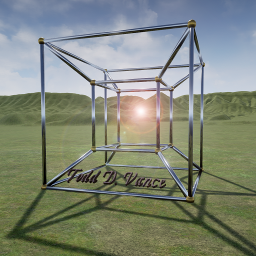
\includegraphics[width=2in]{common/tdv-logo-south-branch-valley-small.png}
  \caption{Hypercube projected into the South Branch Valley}
  \label{fig:logo1}
\end{figure}

\section{Rotations in Three Dimensional Space}

First of all, we need to decide on a coordinate system for three-dimensional space.  A point is a vector of three numbers, $x$, $y$, and $z$.  In Unity, the $y$ axis points up, the $x$ axis points right, and the $z$ axis points directly into the screen (so you are sitting on the negative $z$ axis, and behind the monitor is the positive $z$ axis).  This is an example of a “left-handed system”, which is used largely because graphics card shader languages use that system.  The reason it is a left-handed system is if you take your left hand and make a fist with the  thumb pointing in the positive $z$ direction (I know, it’s awkward), then the fingers will curl along an arc going from the positive $x$ axis through the positive $y$ axis (that is, counterclockwise).  The main advantage of the left-handed system over the right-handed system is if you throw away the $z$ axis, the $x$ and $y$ are in the normal configuration for the two-dimensional plane.

Blender, and mathematicians and engineers most of the time, prefer a right-handed system.  In blender, the $x$ axis comes out of the screen toward you (you sit on the positive $x$ axis, and the negative $x$ axis goes behind the monitor).  The $y$ axis goes to the right.  And, the $z$ axis goes up.  It is right-handed because if you make a fist with your right hand with the thumb pointing up (toward positive $z$), the fingers curl clockwise (looking down) from the positive $x$ axis through the positive $y$ axis.

Let us adopt the convention of a right-handed system for the rest of this document.  Now, we can start looking at rotations.

\section{Euler Angles and Visualizing with a Book}

Take a book.  (Using a book was suggested by mathematician Roger Penrose, because 1. they are common and easy to find, 2. the three different local directions are obvious (as opposed to a sphere or even a spoon), as you will see directly).  Set the (closed) book flat on the table in normal reading configuration--normal, except for being closed of course.  Then, the front cover of the book points upward, in the positive $z$ direction.  You read from left to right, in the direction fof the positive $y$ direction.  And, the text of the book goes from the top of the page to the bottom of the page, in the direction of the positive $z$ direction.   So no matter how you rotate the book, you can see which way, from the book’s point of view, is toward local positive $z$ (from back cover to front cover), toward local positive $y$ (from start of a line to end of a line), and toward local positive $x$ (from the start of a page to the end of a page).

So, again, start with the book, in the “normal” position in front of you as just described, so its local $x$, $y$, and $z$ axes match the global $x$ (toward yourself), $y$ (to the right), and $z$ (toward the ceiling) axes.

There are several ways  to describe a rotation in three dimensional space.  Unreal, Blender, and Unity all use a system of angles about the coordinate axes.  That is, rotation a certain number of degrees about the $x$ axis, a certain number of degrees about the $y$ axis, and a certain number of degrees about the $z$ axis.  Let us try that, and at the same time, notice a problem with the system (that is solved by conventions).

\begin{enumerate}
\item Start with the book in “normal position”.
\item Now, rotate the book 90 degrees clockwise about the $x$ axis.  Thus, it is now resting on its spine with its local $y$ axis pointing toward the ceiling.
\item Next, rotate the book 90 degrees clockwise about the $y$ axis.  Remember, “clockwise” refers to looking down the axis, that is, as a person standing to the right of the book looking at it would see it.  Thus, the book is now upside down, with the spine facing you.
\item Finally, rotate the book 90 degrees clockwise about the $z$ axis.  The book is now upside down with the back cover facing you.
\end{enumerate}

Now, the problem is, what if we did the same three operations in a different order?

\begin{enumerate}
\item Start with the book in “normal position” (i.e., do a “reset” of the book).
\item Now, rotate the book 90 degrees clockwise about the $z$ axis.  It is still sitting on  the table with the front cover facing the ceiling, but the top of the book is to the left. 
\item Next, rotate the book 90 degrees clockwise about the $y$ axis.   It is now sitting on the table with the spine pointing up, but the back cover facing you, and the top pointing to the left.
\item Finally, rotate the book 90 degrees clockwise about the $x$ axis.  The book is now upright with the back cover facing you.
\end{enumerate}

So, the first time, the book ended up upside down with the back cover facing you, and the second time, the book ended up upright with the back cover facing you.  Thus, rotations about axes are \emph{not} commutative operations.  It matters what order you do them in.  So, Blender, Unity, and Unreal have to choose conventions for which axis to rotate about first. This works well in practice, but Mathematicians hate memorizing things so they don’t like having to remember which convention is used.  Not only that, it seems arbitrary to a Mathematician.  Mathematicians like it better when there is a definite natural choice than when you have to follow a man-made convention.  Quaternions solve that, trading elegance for easy understandability for the novice.  Another way to solve that, to be discussed shortly, is the axis-angle scheme, but it has its issues too.

This scheme, incidentally, is called Euler Angles.   In addition to being relatively easy to understand, it has the advantage that it uses exactly three numbers to describe a three-dimensional rotation, and three is the minimum needed (as a mathematician would say, three-dimensional rotation space has three dimensions.  Incidentally, two-dimensional rotation space only has one dimension).  Another advantage is it is similar to a common system for specifying the attitude of an aircraft: yaw, pitch, and roll.  The difference is that with the latter system, local axes are used rather than global axes.

\section{Yaw, Pitch, and Roll}

\section{Axis-Angle Scheme}

\section{Rotation Matrix}








\section{Definition and Formulas}

A quaternion, as the word implies, is a vector of four real (floating point) numbers, such as $(1, 2.5, -5.71, 0)$.  By convention, the previous vector is written as $1 + 2.5i - 5.71j + 0k$, or leaving out the zero coordinate, $1 + 2.5i - 5.71j$.  

When writing software implementing quaternions, the following formulas for addition and multiplication are useful:
\[
(a + bi + cj + dk) + (a’ + b’i + c’j + d’k) = (a+a’) + (b+b’)i + (c+c’)j + (d+d’)k
\]
and
\begin{eqnarray*}
(a + bi + cj + dk)(a’ + b’i + c’j + d’k) &=& aa’ - bb’ - cc’ - dd’  + (ab’ + ba’ + cd’ - dc’)i\\ 
&&+ (ac’ + ca’ - bd’ + db’)j + (ad’ + da’ + bc’ - cb’)k
\end{eqnarray*}

These formulas are good for programming, but not for understanding Quaternions.  For that, one needs to do some algebra.

\section{Algebra of Quaternions}

Recall that real numbers satisfy several algebraic properties: multiplication and addition are commutative, associative, multiplication distributes over addition, and every real number has an additive inverse (its negative), and every nonzero real number has a multiplicative inverse (its reciprocal).

Quaternions satisfy all of these properties that real numbers satisfy, except for one: multiplication is not always commutative.  For example, one can see, using the formula of the last section, that $ij = k$ but $ji = -k$.  That is, $(0+1i+0j+0k)(0+0i+1j+0k)$ $=$ $0(0) - 1(0) - 0(1) - 0(0)$ $+$ $(0(0) +1(0) + 0(0) - 0(1))i$ $+$ $(0(1) + 0(0) - 1(0) + 0(0))j$  $+$ $(0(0) + 0(0) + 1(1) - 0(0))k$ $=$ $k$, but that $(0+0i+1j+0k)(0+1i+0j+0k)$ $=$  $0(0) - 0(1) - 1(0) - 0(0)$ $+$ $(0(1) +0(0) + 1(0) - 0(0))i$ $+$ $(0(0) + 1(0) - 0(0) + 0(1))j$  $+$ $(0(0) + 0(0) + 0(0) -1(1))k$ $=$ $-k$.

William Rowan Hamilton, who invented quaternions, made famous the Quaternion Axiom, which states that $i^2=j^2=k^2=ijk=-1$.  From this, and from all the algebraic properties above (leaving out commutativity of multiplication, except that real (scalar) numbers commute with all quaternions, so for example $2(3i+j)=(3i+j)2 = 6i+2j$)  one can prove the multiplication formula.

In fact, the easiest way to compute with quaternions is to first prove that $ij=k$, $ji=-k$, $jk=i$, $kj=-i$, $ki=j$, and $ik=-j$.  To prove the first one, note that $ijk=-1$ from the axiom, and therefore if you multiply both sides of that equation \emph{on the right} by $k$ (it matters: multiply on the right, not the left), we get $(ijk)k = (-1)k$, and thus $ijk^2=-k$.  But the axiom also states that $k^2=-1$, so we have $ij(-1)=-k$, and since real numbers commute with everything, $-ij=-k$.  Now, just multiply on the left both sides by $-1$, and we get $ij=k$, which was to be proved.  The other five identities are  proven the same way.

Once these are proven, multiplication is just algebra, being careful not to commute things that don’t commute:
\begin{eqnarray*}
(1 - i + 2j)(j - k)&=&(1-i+2j)j + (1-i+2j)(-k)\\
&=&j - ij + 2j^2 + -k + ik + -2jk\\
&=&j - k - 2 - k - j -2i\\
&=&-2-2i-2k
\end{eqnarray*}
and one can check this agrees with the multiplication formula above: $(1 - i + 2j)(j - k)$ $=$ $0 + 0 - 2 + 0$ $+$ 
$(0 + 0 - 2 + 0)i$ $+$ $(1 + 0 - 1 + 0)j$ $+$ $(-1 + 0 + -1 + 0)k$ $=$ $-2-2i-2k$.

\begin{exercise}
Show that 
\begin{eqnarray*}
(a + bi + cj + dk)(a’ + b’i + c’j + d’k) &=& aa’ - bb’ - cc’ - dd’  + (ab’ + ba’ + cd’ - dc’)i\\ 
&&+ (ac’ + ca’ - bd’ + db’)j + (ad’ + da’ + bc’ - cb’)k
\end{eqnarray*}
by multiplying the left hand side while using the algebraic rules (remembering that only real numbers commute with other quaternions) and the rules that $ij=k$, $ji=-k$, $jk=i$, $kj=-i$, $ki=j$, and $ik=-j$.  
\end{exercise}

What about reciprocals? It can be seen that if $q$ is a quaternion $q=a+bi+cj+dk$, and $\bar{q}=a-bi-cj-dk$ is what is called the \emph{conjugate quaternion} to $q$,  then $q\bar{q} = a^2+b^2+c^2+d^2$, which is a real number.  This is straightforward to prove using algebra.  Now, since $q\bar{q}$ is a real number, we can divide by it, as long as it is nonzero.  And it is nonzero exactly when $q$ is nonzero.  Thus, $\frac{q\bar{q}}{q\bar{q}}=1$ if $q\ne{0}$.  This can be rewritten as follows:
\[
q\frac{\bar{q}}{q\bar{q}} = 1
\]
when $q$ is nonzero.  This is another way of saying, $q^{-1} = \frac{\bar{q}}{q\bar{q}}$ or equivalently:
\[
(a+bi+cj+dk)^{-1} = \frac{a-bi-cj-dk}{a^2+b^2+c^2+d^2}
\]
as long as not all of $a$, $b$, $c$, and $d$ are zero.

Finally to divide quaternions, multiply by the reciprocal:  $q/q’ = q(q’)^{-1}$ for right division.  Since multiplication is not commutative, there is a separate “left division” as well: $q’\backslash{q} = (q’)^{-1}q$ by definition.  Note that $q’$ is the denominator even though it appears on the left.

\section{Rotations}
In zero dimensional Euclidean space (a single point), there are no rotations (except the identity rotation, that is, don’t rotate).  In one-dimensional Euclidean space (a line), there are no (non-identity) rotations.  In two-dimensional Euclidean space (a plane), one can rotate by any real number angle (though some real numbers give the same rotation.  For example when the angle is in degrees, a rotation by 90 is the same as a rotation by 450 or by -270 or by any real number of the form $90 + 360n$ where $n$ is an integer.).  Thus, the space of rotations is itself one-dimensional for a plane, but zero-dimensional for a point or a line.  In three dimensions, a rotation can be specified by three Euler angles (plane rotations about the $x$, $y$, and $z$ axes), so the space of rotations is three dimensional in three-dimensional space.  It is hard to see this, but in four dimensional Euclidean space, the space of rotations is six dimensional.  In general, for $n$-dimensional Euclidean space, the space of rotations is $n(n-1)/2$-dimensional.

Thus, for three-dimensional space, three real numbers will specify any rotation (with redundancy, since the rotation by $r+360n$ degrees is the same as the rotation by $r$ degrees for any integer $n$).  But Quaternions have four coordinates, so there is even more redundancy.  The question is, how exactly do Quaternions correspond to Rotations, and why would one prefer that over, say, Euler angles which are at least easier to visualize?

\section{Rules of Quaternion Rotations}
We shall state some basic rules, and then derive properties from these rules.  If $q$ is any quaternion, it represents some rotation in three-dimensional Euclidean space.  But what rotation does it represent?

First of all, if $q$ and $q’$ are quaternions, then the product $qq’$ represents first applying the $q$ rotation, then applying the $q’$ rotation.  This is the main advantage of using quaternions for rotations: combining multiple rotations is an algebraic operation.  This is not the case with Euler angles.

Now, since quaternion rotations combine by multiplication, it goes to reason that the identity rotation (the non-rotation) must be the identity for multiplication, which is $1$, which can also be written $1+0i+0j+0k$.  It also shows that to rotate by the same amount about the same axis in the opposite direction, one would use the reciprocal quaternion: $q^{-1}$ is the inverse rotation to $q$.  

Now, here is where faith comes in.  William Rowen Hamilton realized that the quaternion $i$ represents rotation by 180 degrees about the $x$ axis, the quaternion $j$ represents rotation by 180 degrees about the $y$ axis, and the quaternion $k$ represents rotation by 180 degrees about the $z$ axis.  There are other quaternions representing the same rotation.  For example, it turns out $-i$ is also 180 degrees about the $x$ axis.  

Thus, we have some theorems: rotate 180 degrees about the $x$ axis, then rotation 180 degrees about the $y$ axis.  If you do this, the effect is the same as rotating 180 degrees about the $z$ axis, because $ij=k$.    Try it with some object like a book and you will see this is true.  Let us use the Blender standard (different from the Unity standard) of $x$ being forward ( positive) and back (negative), $y$ being right (positive) and left (negative), and $z$ being up (positive) and down (negative.  Hold a book so that the front cover faces away you and is upright, that is in the positive $x$ direction.  If you rotate it 180 degrees about the $x$ axis, the front cover still faces away from you, but it is now upside down.  If you rotate it 180 degrees about the $y$ axis, the front cover is now facing you and is upright.  This is the same thing that would have happened if you started with the book upright, front cover facing away from you, then rotated it 180 degrees about the $z$ axis.

So, we now know how to make the nonrotation and the 180 degree rotations about the coordinate axes into quaternions: $1$, $i$, $j$, and $k$.  Let us try to deduce another one.  For example, what quaternion would represent a 90-degree rotation about the $x$ axis?

\section{Square Roots of Quaternions}

We need some quaternion $q$ that we want to represent rotation by 90 degrees about the $x$ axis.  If we apply $q$ twice, that’s the same as applying $i$, a rotation of 180 degrees about the $x$ axis.  Thus, $q$ is a solution to the equation $q^2 = i$.  Can we find just one solution?

Let $q=a+bi+cj+dk$.  Then, using algebra (or you could use the multiplication formula), 
\begin{eqnarray*}
q^2 &=& (a+bi+cj+dk)(a+bi+cj+dk)\\
&=&a^2 +abi + acj + adk + bai - b^2 +bck - bdj + caj - cbk - c^2 +cdi + dak + dbj - dci - d^2\\
&=&a^2-b^2-c^2-d^2 + (ab+ba+cd-dc)i + (ac-bd+ca+db)j + (ad+bc-cb +da)k
\end{eqnarray*}
which must equal $i$, so we have the following system of four quadratic equations in four variables:
\begin{eqnarray*}
a^2-b^2-c^2-d^2 &=&0\\
2ab&=&1\\
2ac&=&0\\
2ad&=&0
\end{eqnarray*}
So, neither $a$ nor $b$ is 0 since $ab=\frac12$.  This implies $c$ and $d$ are both 0 since $ac=ad=0$ and $a$ is nonzero.
Thus the equations are reduced to:
\begin{eqnarray*}
a^2&=&b^2\\
2ab&=&1\\
\end{eqnarray*}
So, $a=\pm{b}$.

If $a=b$, then $2ab=1$ means $a^2=\frac12$, so $a=\sqrt{2}{2}=b$ or $a=-\sqrt{2}{2}=b$
If $a=-b$, then $-2a^2=1$ so $a$ is not even real.  So, this means:
\[
q=\sqrt{2}2 + \sqrt{2}2i
\]
or
\[
q=-\sqrt{2}2 - \sqrt{2}2i
\]
One  of these corresponds to clockwise rotation by 90 degrees, the other counterclockwise rotation by 90 degrees.  It is only a matter of convention which is which, as long as that convention is consistant.

In theory, one can do a lot of algebra and compute, say, a 180th root of $i$ to get rotation by one degree.   There is an issue that there could be 180 180th roots of $i$ and in Quaternion algebra, there can easily be more (or less if there are multiple roots).  But suppose $d$ is a quaternion that is a 180th root of $i$.  Then, $d^{180}=i$, so doing this rotation 180 times gives a 180 degree rotation.  Therefore, no matter which root is chosen, it is a rotation of degree 1 about the $x$ axis in some direction, either clockwise or counterclockwise.  Thus, in theory, we can represent any rotation as a quaternion based on the information given so far.

In fact, one way to do this is the following plan (which can be a hard project for someone really interested):

\begin{enumerate}
\item Find a formula for the square root of \emph{any} quaternion $a+bi+cj+dk$ by setting up a system and trying to solve it.  This is not really all that easy.
\item Write code to implement the square root function for quaternions.  Let us say the function $f(q)$ returns a value such that $f(q)^2=q$.  There is more than one choice of value, of course.  Let us say that we choose one whose $a$ coefficient is positive.  If there is none (this happens if the $a$ coefficient is zero on all solutions), choose one where the $b$ coefficient is positive.  Again if there is none, choose one where the $c$ coefficient is positive.  If there is none, choose one where the $d$ coefficient is positive.  If there is none, then we are taking the square root of 0 and the answer is 0.
\item Let $a_0=i$ and let $a_1=\sqrt{2}2=f(i)$.  Then for each $n>1$, let $a_n=f(a_{n-1})$ up to some number, say 64.  Then $a_n$ is rotation by the angle $\frac{180}{2^n}$.  By scaling the angle by $\frac{1}{180}$ and writing the angle in floating point binary, one can convert any angle $\theta$ to a sum of reciprocal powers of 2.  This shows how to multiply the $a_i$ to produce the quaternion representing rotation by that angle about the $x$ axis.
\item Do the analogous for the $y$ and $z$ axis.
\end{enumerate}

\section{Giving Away the Answer}
In practice, a lot of work has already been done and it’s simpler (and safer: fewer mistakes) to use known, tested formulas when writing software.  The Wikipedia article \url{https://en.wikipedia.org/wiki/Quaternions_and_spatial_rotation} discusses this.

If we want to rotate by an angle $\theta$ about the axis defined by the vector $(a,b,c)$ (for example, the $x$ axis is $(1,0,0)$), first ensure the vector is a unit vector: replace $(a,b,c)$ with $(a/m,b/m,c/m)$ where $m=\sqrt{a^2+b^2+c^2}$.

Then, the quaternion representing the rotation is 
\[q=e^{\frac12\theta(\frac{a}{m}i+\frac{b}{m}j+\frac{c}{m}k)}.\]
 We now need to find out how to compute the exponential function of a quaternion.

This is a well-established formula:
\[
e^{\frac12\theta(\frac{a}{m}i+\frac{b}{m}j+\frac{c}{m}k)}=\cos{\frac{\theta}2} + (\frac{a}{m}i+\frac{b}{m}j+\frac{c}{m}k)sin{\frac{\theta}2}
\]
which works because $(a/m,b/m,c/m)$ is a unit vector.

\section{Applying Quaternions to Points}
Suppose we have a geometric configuration defined by points $p=(x,y,z)$. How do we use a quaternion to rotate that point?

To rotate the configuration about the origin $(0,0,0)$, take the rotation quaternion $q$ and for each point $p=(x,y,z)$ defining the configuration, compute the following: $w’+x’i+y’j_z’k = q(xi+yj+zk)q^{-1}$.  Then, the point $p$ is mapped to the new point $p’=(x’,y’,z)’$, where we just throw away $w’$.

For more general rotations about some central point $c$, just take the vector $p-c$, rotate it about the origin to get $p’$, then the point you want is $p’+c$.  This is a common pattern in mathematics: to solve a new problem, first translate it to a known problem domain (that is, one whose solution method is already known), solve the known problem, then translate it back to the new problem domain.

\section{Extracting the rotation from a quaternion}
By reversing the process above, we can find the axis and the angle given a quaternion.  Suppose we have a rotational quaternion $q=a+bi+cj+dk$.  

Let $m’=\sqrt{a^2+b^2+c^2+d^2}$.  It can be shown with trigonometry that  if $q$ came from the exponential formula above, then $m’$ would be 1.  In general, we work  with $q’=q/m’$ to force this to be the case.  Thus, 
$q’=\frac{a}{m’}+\frac{b}{m’}i+\frac{c}{m’}k+\frac{d}{m’}k$.

The axis that the rotation goes about is the vector:
$(b/m, c/m, d/m)$ where $m=\frac{\sqrt{a^2+b^2+c^2}}{m’}$.
Then, $Y=m=\sin\frac{\theta}{2}$ and $X=\frac{a}{m’}=\cos\frac{theta}{2}$.  Therefore, the $\mathrm{atan2}$ function, available in many programming languages, can be used to extract the angle from $X$ and $Y$.


















\end{document}